%& -job-name=Assignment4
\input{./documents-common/preamble.tex}
\begin{document}
  \maketitle[Computational Finance]{Pricing of Barrier Options using Finite Differences}
%TODO: small bit about their use
\section{Barrier Options}
Barrier options are options which either come into play or drop-out if the $S$ hits
a predefined value.
We have investigated and will discuss {\em up-and-out call options}, which are options which expire
worthless when the underlying assets hits a predefined top-barrier. These types of options can be used to
hedge ones risks when taking a short position, and of course speculatatively.
\par We will show how to model this type of option using a discrete PDE and compare it to a vanilla option.
  \section{Methodology}
  In order to calculate the value of a up-and-out European barrier-option we use a finite-difference approximation of the Black-Scholes model.
  This model is given by:
  \begin{align}
    \label{eq:pde}
    \pdrv[t]V + rS\pdrv[S]V + \frac{1}{2}\sigma^2S^2\pdrv[S^2]{^2V}-rV = 0
 \end{align}
 We discretize it in $S$ space using a standard equidistant grid and the standard second-order central finite-difference methods for the derivatives.
 That is,
 \begin{align}
   \pdrv[S]V &= \frac{V(t, S+\Delta S)-V(t, S-\Delta S)}{2\Delta S},\nn
   \pdrv[S^2]{^2V} &= \frac{V(t,S+\Delta S)-2V(t,S)+V(t,S-\Delta S)}{\Delta S^2}
 \end{align}
 We Discretize in time by making the change of variable $t\to \tau, \tau = T-t$ and integrate using the BDF-2 scheme.
 The BDF-2 scheme is given by
 \begin{align}
  &V^+ - \frac{4}{3}V + \frac{1}{3}V^- = \frac{2}{3}\Delta t A V^+\nn
  \to& \left(3I-2\Delta t A)V^+ = 4V-V^-
 \end{align}
 Where $A$ is a tridiagonal matrix constructed using the finite-difference scheme we showed before.

\subsection{Initial Conditions}
 For the initial condition we use $(V-K)^+$ just as we did before.

 \subsection{Boundary Conditions}
  The boundary conditions on a up-and-out barrier option are given by
  \begin{align}
    V(S > \text{barrier}) = V(S < K) = 0.
  \end{align}
  This is easy to understand intuitively, as these are the conditions imposed on us by the definition of the barrier and the pay-off function respectively.

  We use the injection method to implement these boundary conditions (i.e. we forcefully set the boundaries to zero after each update).
\section{Results}
\begin{figure}[h!]
  \caption{}
  \centering
    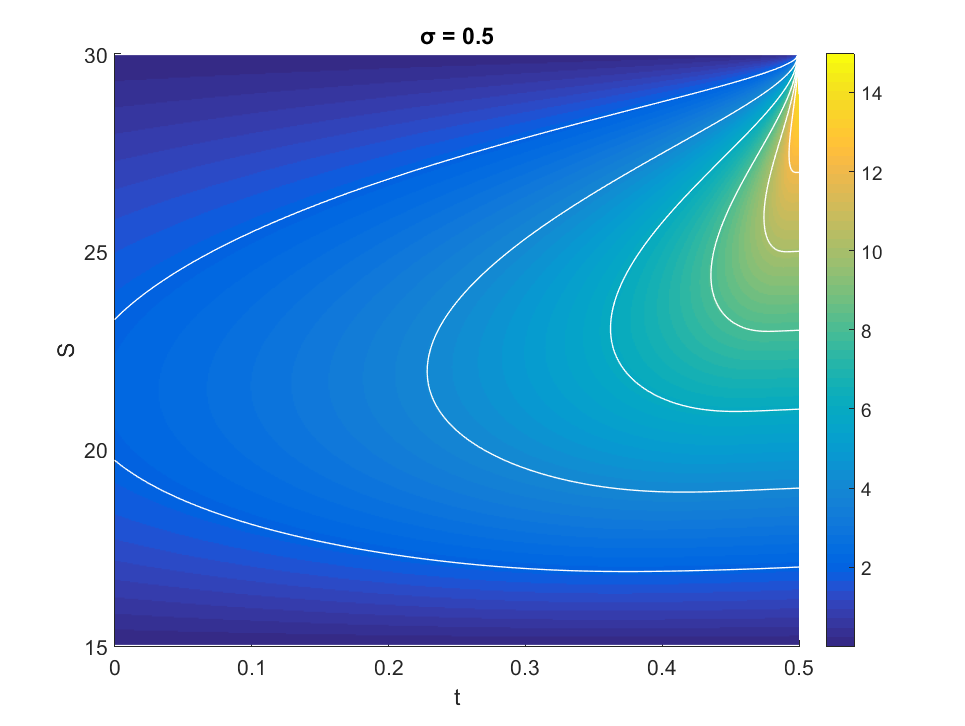
\includegraphics[width=0.75\textwidth]{plots/field}
    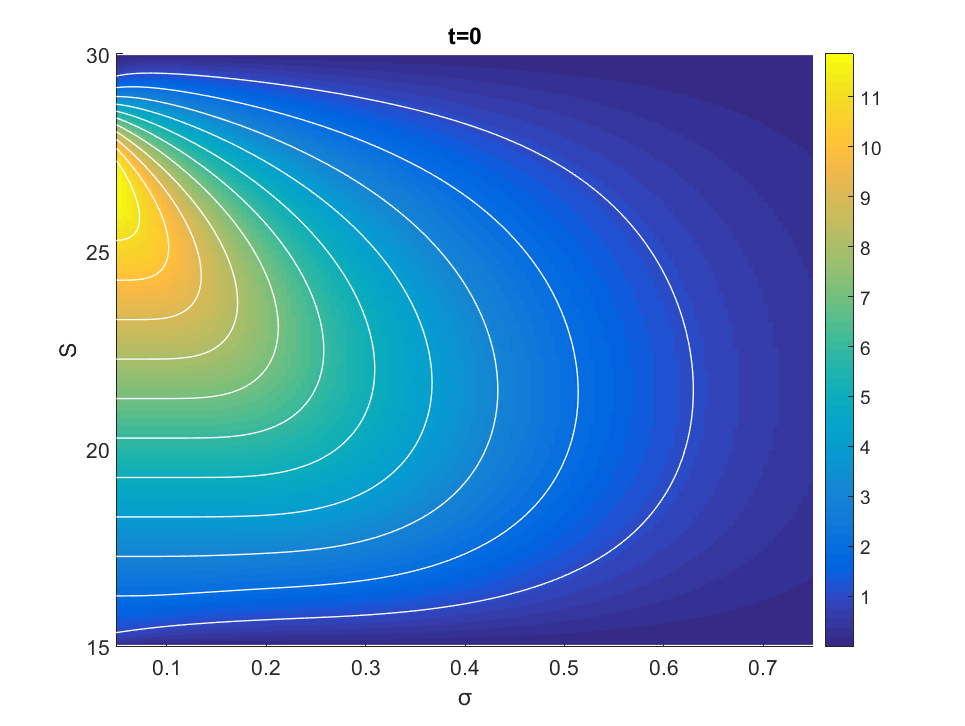
\includegraphics[width=0.75\textwidth]{plots/sigma_field}
\end{figure}
Note how $V$ curves with $S$ along the time axis, and how a lower volatility leads to an increased value as opposed to the opposite.
intuitively this is because for a normal option there is a broken symmetry between a swing up and a swing down. A swing up always means more profit, but a swing down can never go below zero.
Here a swing up can also lead to reduced profits, returning some symmetry but once it hits the top barrier it will expire worthless. Therefor a lower volatility is preffered because it reduces the odds
of hitting the barrier.
  \subsection{The Greeks}
  The greeks can be computed by taking the finite-difference derivatives with respect to dependant variables.
  The greeks we will look at are given by
  \begin{align}
    \Delta = \pdrv[S]V,\nn
    \nu = \pdrv[\sigma]{V}.
  \end{align}
  They can be computed using the standard finite difference approximations we showed before. We will compare these to the results we previously obtained for standard European options.
  \subsubsection{$\Delta$}
  Delta is a measure of the rate of change in the value $V$ as function of $S$. We can compute it by taking the derivative of our computed solutions w.r.t. to $S$
  We have plotted it in figure \ref{fig:delta}. Note how both display singularities near the borders but have an oherwise smooth surface with a seamingly linear divide between positive $\Delta$ and negative $\Delta$.
  \begin{figure}[hhp!]
    \caption{}
    \label{fig:delta}
    \centering
      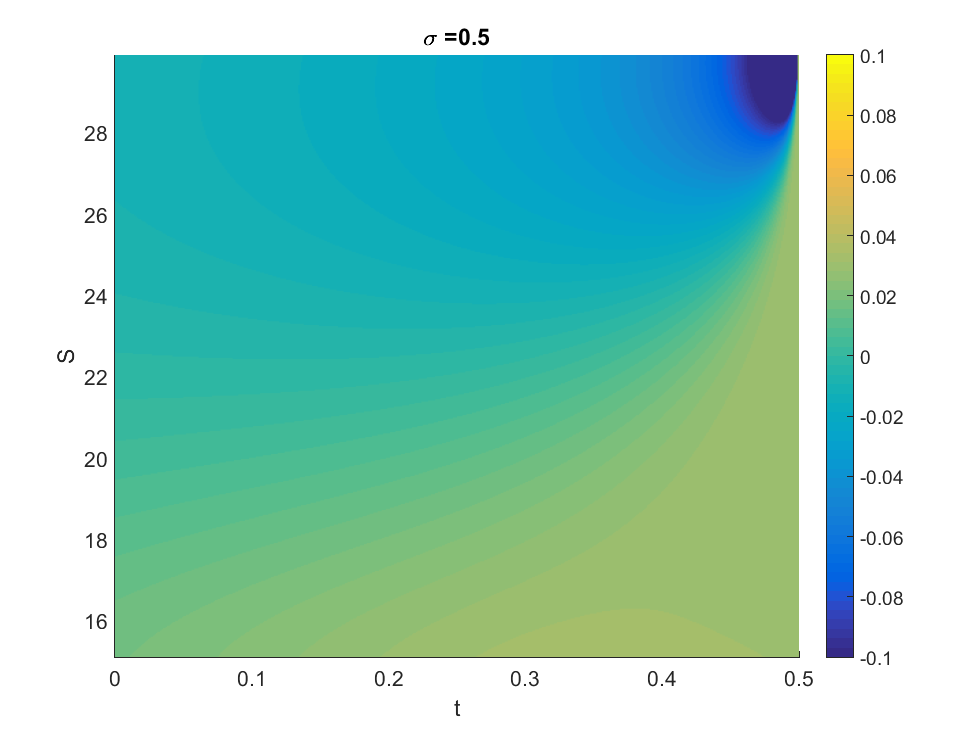
\includegraphics[width=0.75\textwidth]{plots/delta_field}
      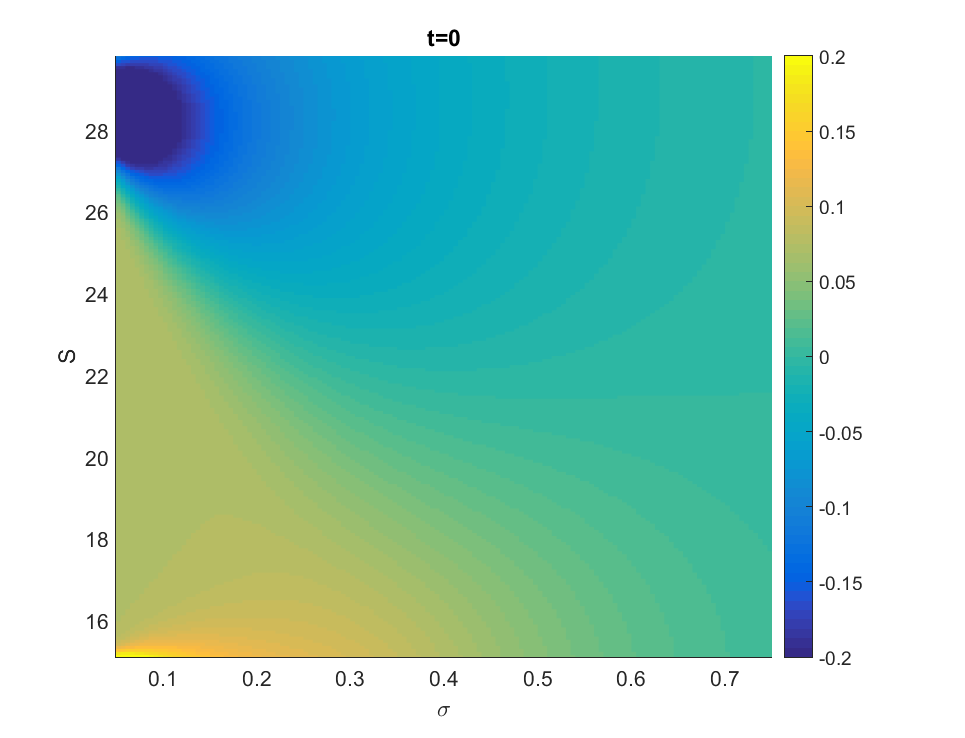
\includegraphics[width=0.75\textwidth]{plots/delta_sigma_field}
  \end{figure}
  \subsubsection{$\nu$}
  Vega is a measure of how the value of an option changes with the implied volatility of the underlying asset. We have computed the value $\nu$ at time $t=0$ for various
  values of sigma, as shown in figure \ref{fig:nu}. This figure is not too surprising looking at the previous image of $V$ versus $\sigma$.
  \begin{figure}[hhp!]
    \caption{}
    \label{fig:nu}
    \centering
      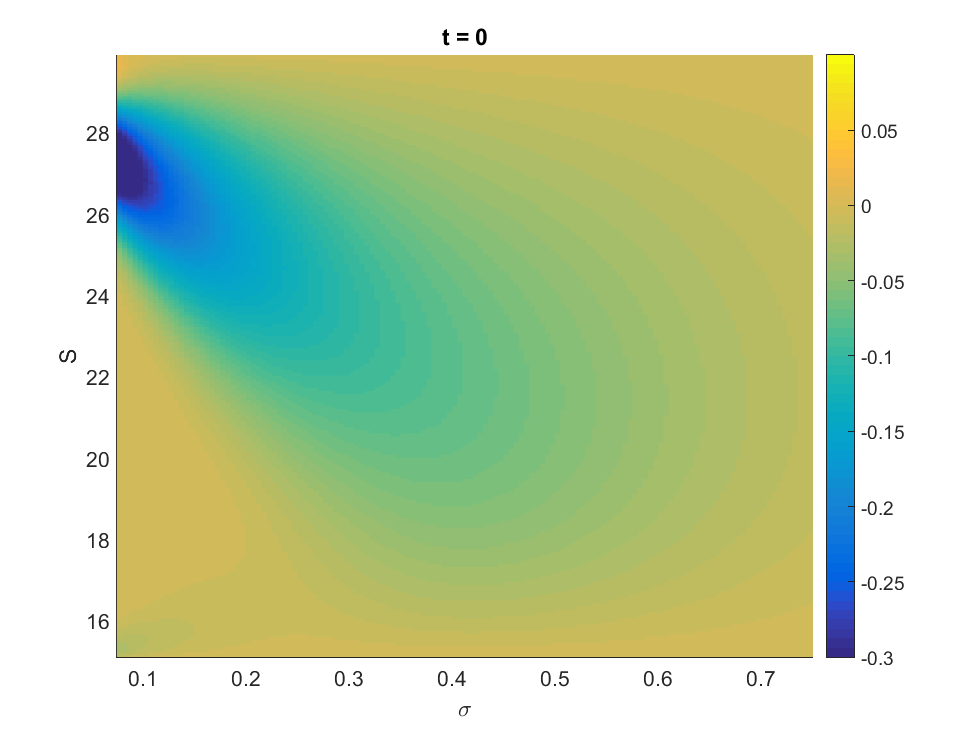
\includegraphics[width=0.75\textwidth]{plots/vega_field_sigma}
  \end{figure}

  %TODO: Ask what would be better, vega as a function of T or vega as a function of S? both?

\end{document}
